%!TEX root = /Users/Nikolaj/Developer/GPU-Project/Report/Report.tex

\subsection{Architecture}
In a traditional computer, CPUs and GPUs coexist as the processing units of the computer and the graphics chip respectively. Historically, the graphics chip has been used to render games and images on screen while the CPU is responsible for a lot of administrative tasks like executing the operating system and the processes running on it. Besides a great deal of floating point operations (flops) this requires that it communicates with other parts of the system through channels that might suffer from high latency which introduces the need for caching. Since caching is a vital function for the CPU it also occupies a lot of chip area, leaving fewer transistors for arithmetic logical units (ALU) to do actual arithmetic operations. \\

Conversely, a large number of ALUs is what makes the GPU effective in doing its job because pixel rendering requires a lot of flops per second to create a smooth graphical user experience. Where the CPU uses large caches to hide latency from other hardware units, where the GPU makes use of warps and small caches to hide latency from read and write operations. The concept of warps will be discussed later in Section \ref{sec:kernelandwarps}.

\centerline{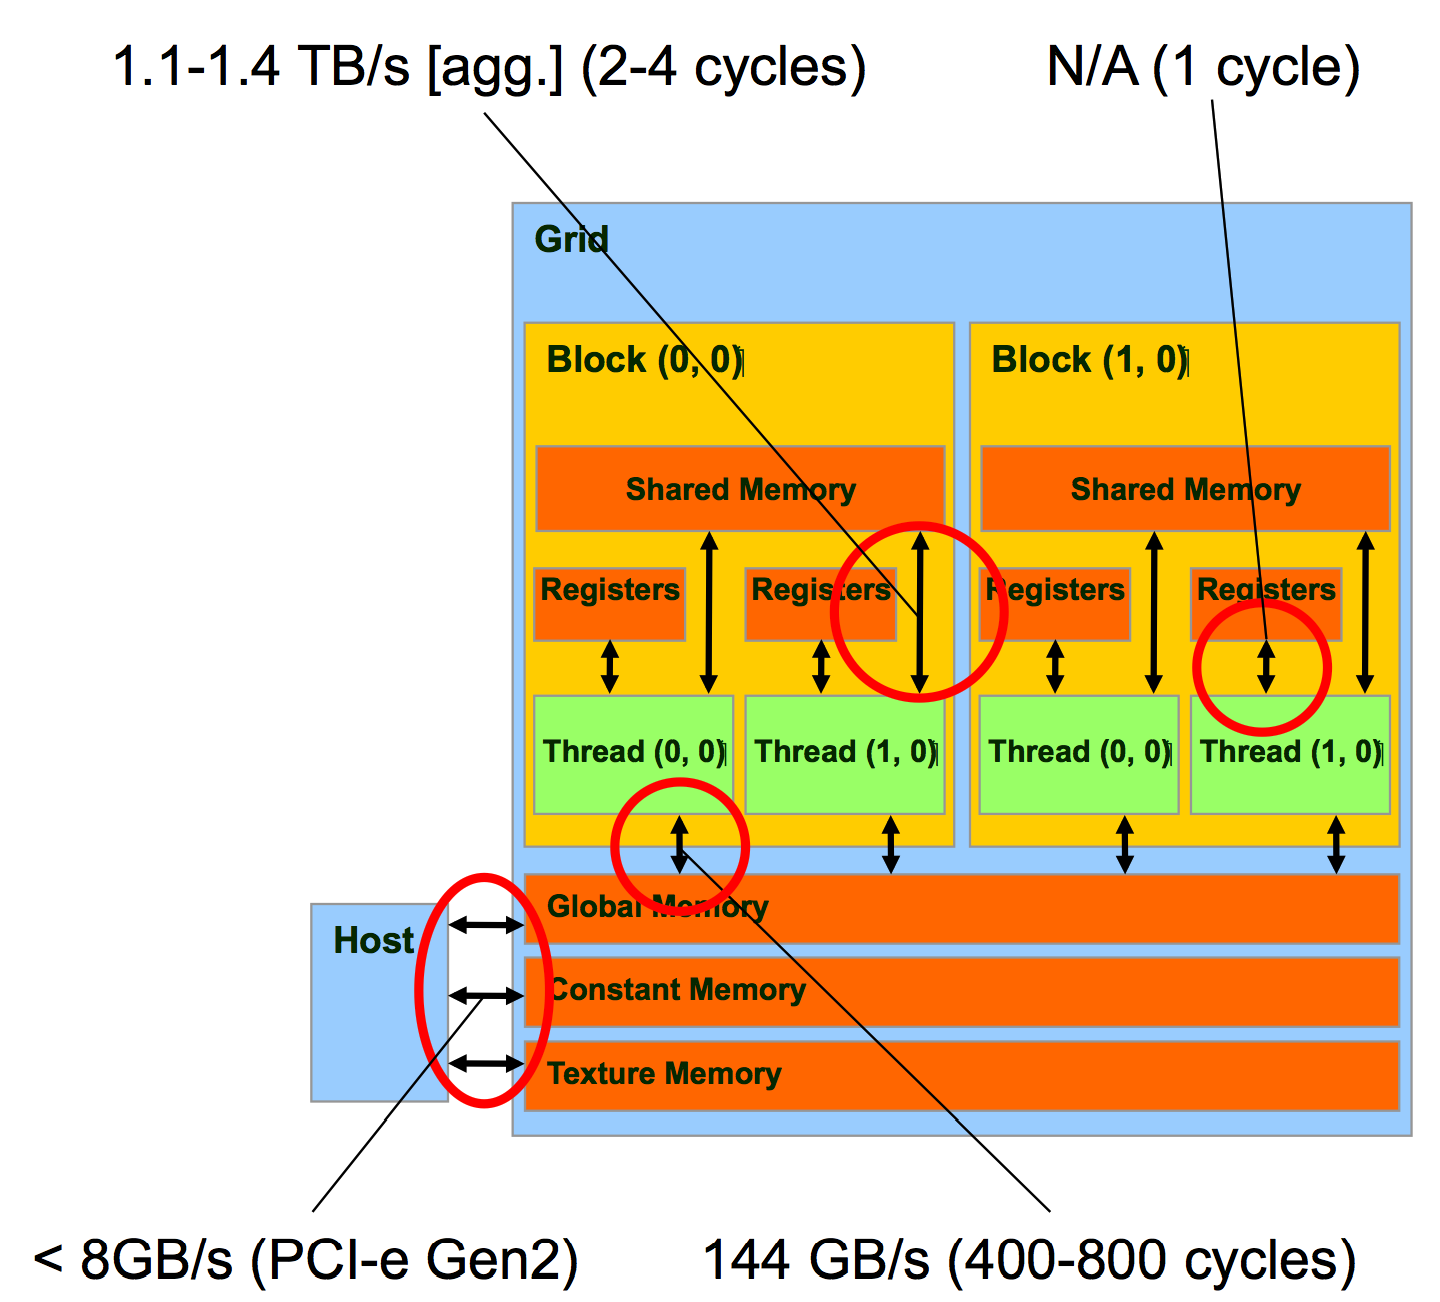
\includegraphics[width=\textwidth]{img/latenstid.png}} 
%The GPU never directly communicates with devices, like the hard drive, but gets its data from on-board memory areas so it does not need a large cache area.\\

Compute Unified Device Architecture (CUDA) is a parallel computing model created by Nvidia in 2006 based on an extension of the C programming language \cite{pmpp}. In a CUDA enabled computing system, the CPU is known as the \emph{host} and GPU(s) are known as \emph{devices}. CUDA programs are executed on the system as whole, meaning that the host and the device cooperate on computing the output. This is advantageous because some computing tasks are only partially suited for parallelization, meaning that such tasks should be split in smaller parts and executed separately on the most favourable piece of hardware for maximum efficiency.\\

The entry point of a program is always a procedure executed by the host. When the execution is started, the host is instructed to delegate suitable parts of the task to one or several devices embedded as code blocks in \emph{kernels} which is the CUDA term for a function executed on a device. If the task computed by the kernel operates on external data, that data must be copied (by the host) into device memory before the kernel is invoked. Likewise, when the kernel terminates, the host is responsible for reading the data back and deallocate the memory areas used.\\

\subsection{Streaming Multiprocessors}
The computing resources of the GPU is divided into a number of streaming multiprocessors (SMP) each responsible for scheduling a number of threads. Typically, the GPU as a whole executes thousands of threads in parallel split between a number of SMPs. Each thread is much more lightweight than normal CPU threads and typically take only a few clock cycles to create and schedule compared to several thousands of cycles on normal CPUs. Thus, thread context switching is a very efficient operation. Other than that, CUDA threads are similar to regular CPU threads with registers etc. All threads execute the same kernel simultaneously but work on different pieces of the data following the ``Single Program Multiple Data'' (SPMD) paradigm in contrast to CPU threads that are programmed separately. \\

\subsection{Blocks}
Since a kernel is executed by up to millions of threads and each SMP has an upper limit on the number of threads it can execute at a time, SMPs load threads in groups called blocks. Threads within a block can communicate through the shared memory region and will always be executed by the same SMP once assigned. Other examples of properties for thread blocks include synchronization, whereby the threads in the block can be synchronized to wait for each other at a specific place in the kernel code. The capacity of an SMP is limited both in terms of threads and in terms of blocks. E.g if a block contains 128 threads, the SMP has room for 8 blocks, and if the block contains 256 threads, the SMP has room for only 4 blocks.

\subsection{Kernel Invocation and Warps}
\label{sec:kernelandwarps}
When a kernel is invoked, the user specifies two parameters enclosed in angle brackets before the parameter list. The first parameter sets the number of blocks that should be available for the execution of the kernel. The second parameter sets the number of threads in each block. The configuration of threads and blocks is normally referred to as the kernel grid because each block is identified by three numbers corresponding to coordinates in a 3-dimensional grid. Likewise each thread is identified within a block using three thread coordinates. These identifiers are all available in code through predefined variables and can be used to distinguish threads from each other when selecting data for the thread to operate on.\\

When a number of blocks from the grid are loaded by an SMP, the threads of each block are further split into units of 32 threads called warps which is the smallest unit of execution in the sense that all threads from the same warp always execute the same instruction. After some time, one or several blocks are put aside and leave room for new blocks to fill the gap. The user is left without tools to choose which blocks should be loaded, in which order and for how long time the blocks should be executed before new blocks take their place. This is all scheduled by the hardware which gives the CUDA programs the strength that programs can be moved between different machines with different GPUs and automatically utilize the hardware available without changing the source code. The more SMPs available on the chip, the more blocks and threads can execute in parallel.

All threads within the same warp share the same execution path at any given time. In case of conditional statements where the threads would enter different parts of the condition, \emph{branch divergence} happens. This effectively means that the warp will execute each part of the code that the different threads enter. If all threads enter the same branch, branch divergence does not happen.

\subsection{Memory}
A CUDA device exposes different kinds of memory with each their latency and access scope. Since latency has a direct influence on performance, considering which types of memory is used in a CUDA program is important to utilize the full performance potential. Besides latency issues, blocks in an SMP might use more shared memory than is available in which case the number of blocks will be automatically reduced, thus affecting the overall performance of the program. \\

The memory model in CUDA is shown in Fig. XX(INSERT FIGURE). The figure shows a grid of threads divided into two blocks with two threads each. Memory types include constant memory, global memory, shared memory and thread registers. Global- and constant memory are the only memory types that can be accessed from the host. These are the places where the host can store data to be used in kernel code using CUDA functions similar to memory management functions from C. The kernel threads can then access the data directly using their block- and/or thread IDs. Constant memory is read only from the device, but is much faster to read from compared to global memory. The results from the kernel is written to global memory, since it is the only place the device can write to and the host can read from, where it can be copied back to the host.\\

Global memory suffers from high latency and has a risk for slowing down the kernel execution if not used carefully. This is partly made up for by the constant memory which is slightly faster but read-only by the device. Shared memory and thread registers on the other hand are extremely fast compared to all other memory types(Insæt memory latency figur). Shared memory is private to each block, limited in size and offers a mean for threads in the block to communicate by writing intermediate results from their computation where other threads can reach them. Thread registers are private to each thread and is used to store frequently accessed data that does not need to be accessed by other threads. Keywords and functions exist in CUDA C to allocate/deallocate memory and declare a variable as residing in either of the memory types which directly defines the accessibility of the variable to other threads.